%%%%%%%%%%%%%%%%%%%%%%%%%%%%%%%%%%%%%%%%%%%%%%%%%%%%%%%%%%%%%%%%%%%%%%%%%%%%%%%%%%
\begin{frame}[fragile]\frametitle{}
\begin{center}
{\Large Ensemble}
\end{center}
\end{frame}


%%%%%%%%%%%%%%%%%%%%%%%%%%%%%%%%%%%%%%%%%%%%%%%%%%%%%%%%%%
\begin{frame}[fragile]\frametitle{For Complex Decision Making}
\begin{itemize}
\item How do I handle data for large number of variables?
\item More complex the decision making, more experts are needed.
\item  Linux, for example, is such a complex system that building it took hundreds of experts.
\item Ensemble means collection of models, meaning collection of experts!!
\end{itemize}
\end{frame}

%%%%%%%%%%%%%%%%%%%%%%%%%%%%%%%%%%%%%%%%%%%%%%%%%%%%%%%%%%
\begin{frame}[fragile]\frametitle{What is Ensemble?}
\begin{itemize}
\item Definition: An ensemble is a set of elements that collectively contribute to a whole. 
\item A familiar example is a musical ensemble, which blends the sounds of several musical instruments to create a beautiful harmony, or architectural ensembles, which are a set of buildings designed as a unit. 
\item In ensembles, the (whole) harmonious outcome is more important than the performance of any individual part.
\end{itemize}
\end{frame}

%%%%%%%%%%%%%%%%%%%%%%%%%%%%%%%%%%%%%%%%%%%%%%%%%%%%%%%%%%
\begin{frame}[fragile]\frametitle{Theorem about Ensemble}
\begin{itemize}
\item Condorcet's jury theorem (1784) is about an ensemble in some sense. 
\item It states that, if each member of the jury makes an independent judgment and the probability of the correct decision by each juror is more than 0.5, then the probability of the correct decision by the whole jury increases with the total number of jurors and tends to one. 
\item On the other hand, if the probability of being right is less than 0.5 for each juror, then the probability of the correct decision by the whole jury decreases with the number of jurors and tends to zero.
\end{itemize}
\end{frame}

%%%%%%%%%%%%%%%%%%%%%%%%%%%%%%%%%%%%%%%%%%%%%%%%%%%%%%%%%%
\begin{frame}[fragile]\frametitle{Idea behind Ensemble}
\begin{itemize}
\item Rational: `No Free Lunch' Theorem: Even popular base classifiers will perform poorly on some datasets, where the learning classifier and data distribution do not match well
\item Intuitive Justification: When combing multiple, independent, and diverse, decisions each of
which is at least more accurate than random guessing then random errors cancel each other out, and correct decisions are reinforced
\end{itemize}
\end{frame}

%%%%%%%%%%%%%%%%%%%%%%%%%%%%%%%%%%%%%%%%%%%%%%%%%%%%%%%%%%
\begin{frame}[fragile]\frametitle{Idea behind Ensemble}
\begin{itemize}
\item 5 classifiers each with 0.7 accuracy. 
\item All of them give predictions. 
\item Some match , some don't.
\item Majority voting means $>= 3$ should be correct. So when all 5 or 4 or 3 are correct.
\end{itemize}

\begin{center}
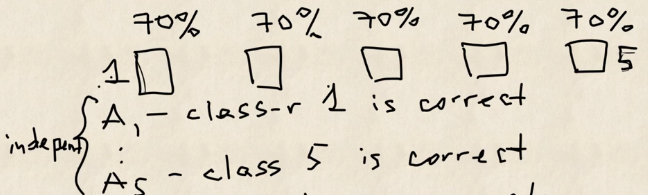
\includegraphics[width=0.8\linewidth,keepaspectratio]{ens10}
\end{center}


\end{frame}

%%%%%%%%%%%%%%%%%%%%%%%%%%%%%%%%%%%%%%%%%%%%%%%%%%%%%%%%%%
\begin{frame}[fragile]\frametitle{Idea behind Ensemble}
\begin{itemize}
\item Probability that all 5 classifiers would be correct is $ (0.7) * (0.7) \ldots = (0.7)^5$

\item Probability that 4 classifiers would be correct and one incorrect is $(0.7)^4  \times (0.3)^1$
\item Binomial theorems says that as there are ${1 \choose 5}$ arrangements of this are possible. See, the incorrect one can be any one of the 5. So the probability is ${1 \choose 5} (0.7)^4  \times (0.3)^1$
\item Probability that 3 classifiers would be correct and two incorrect is ${2 \choose 5}  (0.7)^3 \times (0.3)^2$

\item Total probability is to add them up = $(0.7)^5 + {1 \choose 5} (0.7)^4  \times (0.3)^1 + {2 \choose 5} (0.7)^3 \times (0.3)^2 \approx 0.84$
\end{itemize}
Did you see? Individually they were 0.7 each, but together 0.84!!! If we take $N = 1000$ classifiers, then the total accuracy goes to 0.99
\end{frame}




%%%%%%%%%%%%%%%%%%%%%%%%%%%%%%%%%%%%%%%%%%%%%%%%%%%%%%%%%%
\begin{frame}[fragile]\frametitle{Jury to Ensemble?}

$\mu = \sum_{i=m}^{N}{N\choose i}p^i(1-p)^{N-i}$

Where,
\begin{itemize}
\item $N$ is the total number of jurors;
\item $m$ is a minimal number of jurors that would make a majority, that is $m = \frac{N + 1}{2}$;
\item ${N \choose i}$ is the number of i-combinations from a set with $N$ elements.
\item $p$ is the probability of the correct decision by a juror;
\item $\mu$ is the probability of the correct decision by the whole jury.
\end{itemize}

It can be seen that if $p>0.5$, then $\mu >p$. In addition, if $N \rightarrow \infty$, then $\mu \rightarrow 1$.
\end{frame}

%%%%%%%%%%%%%%%%%%%%%%%%%%%%%%%%%%%%%%%%%%%%%%%%%%%%%%%%%%
\begin{frame}[fragile]\frametitle{Wisdom of the crowd}
\begin{itemize}
\item In 1906, Francis Galton visited a country fair in Plymouth where he saw a contest being held for farmers. 
\item  800 participants tried to estimate the weight of a slaughtered bull. 
\item  The real weight of the bull was 1198 pounds. Although none of the farmers could guess the exact weight of the animal, the average of their predictions was 1197 pounds.
\end{itemize}
A similar idea for error reduction is adopted in the field of Machine Learning, called Ensemble.

\end{frame}


%%%%%%%%%%%%%%%%%%%%%%%%%%%%%%%%%%%%%%%%%%%%%%%%%%%%%%%%%%
\begin{frame}[fragile]\frametitle{Ensemble Rationale}
Another Example:
\begin{itemize}
\item Assume we have 25 binary classifiers
\item Each has error rate: $\epsilon$= 0.35
\item If all 25 classifiers are identical:
\item They will vote the same way on each test instance.
\item Majority wins, so the max one, which is $\epsilon$= 0.35 is the final answer.
% \item Ensemble error rate: $\epsilon$= 0.35
\end{itemize}
\end{frame}

%%%%%%%%%%%%%%%%%%%%%%%%%%%%%%%%%%%%%%%%%%%%%%%%%%%%%%%%%%
\begin{frame}[fragile]\frametitle{Ensemble Rationale}
\begin{itemize}
\item Ensemble method only makes a wrong prediction if more than half of the base classifiers predict incorrectly.
\item The probability that the ensemble classifier make's a wrong prediction (for half the set, ie from 13 to 25) is, binomial, ie:
\begin{center}
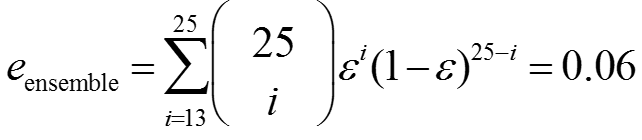
\includegraphics[width=0.6\linewidth,keepaspectratio]{ensmerr}
\end{center}
\item 6\% much less than 35\%

\end{itemize}
{\tiny (Ref: ``A Survey of Ensemble Classification - SMU'', ``Tan, Steinbach , and Kumar'')}
\end{frame}

%%%%%%%%%%%%%%%%%%%%%%%%%%%%%%%%%%%%%%%%%%%%%%%%%%%%%%%%%%
\begin{frame}[fragile]\frametitle{Ensemble Rationale}
Conditions necessary for an ensemble classifier to perform better than a single classifier:
\begin{itemize}

\item Base classifiers should be independent of each other
\item Base classifiers should not do worse than a classifier doing random guessing
\item Example: for two-class problem, base classifier error rate: $\epsilon< .5$

\end{itemize}
\end{frame}

%%%%%%%%%%%%%%%%%%%%%%%%%%%%%%%%%%%%%%%%%%%%%%%%%%%%%%%%%%
\begin{frame}[fragile]\frametitle{When to Ensemble?}
\begin{itemize}
\item Given a fixed-size number of training samples, our model will increasingly suffer from the ``curse of dimensionality'' if we increase the number of features.
\item The challenge of individual, un-pruned decision trees is that the model often ends up being too complex for the underlying training data -- decision trees are prone to over-fitting.
\end{itemize}
\end{frame}




%%%%%%%%%%%%%%%%%%%%%%%%%%%%%%%%%%%%%%%%%%%%%%%%%%%%%%%%%%
\begin{frame}[fragile]\frametitle{For Complex Decision Making}
\begin{itemize}
\item Ensemble are called as``meta-algorithms'': approaches to combine several machine learning techniques into one predictive model
\item Bagging and random forests are ``bagging'' algorithms that aim to reduce the complexity of models that overfit the training data.
\item In contrast, boosting is an approach to increase the complexity of models that suffer from high bias, that is, models that underfit the training data.
\end{itemize}
\end{frame}

%%%%%%%%%%%%%%%%%%%%%%%%%%%%%%%%%%%%%%%%%%%%%%%%%%%%%%%%%%
\begin{frame}[fragile]\frametitle{Ensemble Characteristics}
\begin{itemize}
\item Build multiple models from the same training data by creating each model on a modified version of the training data.
\item Make a final, ensemble prediction by aggregating the predictions of the individual models
\item Classification prediction: Let each model have a vote on the correct class prediction. Assign the class with the most votes.
\item Regression prediction: Measure of central tendency (mean or median)
\end{itemize}
\end{frame}



%%%%%%%%%%%%%%%%%%%%%%%%%%%%%%%%%%%%%%%%%%%%%%%%%%%%%%%%%%
\begin{frame}[fragile]\frametitle{Ensemble Constructing}
\begin{itemize}
\item By manipulating the training set.
\item By manipulating the input features.
\item By manipulating the class labels.
\item By manipulating the learning algorithm.
\end{itemize}
\begin{center}
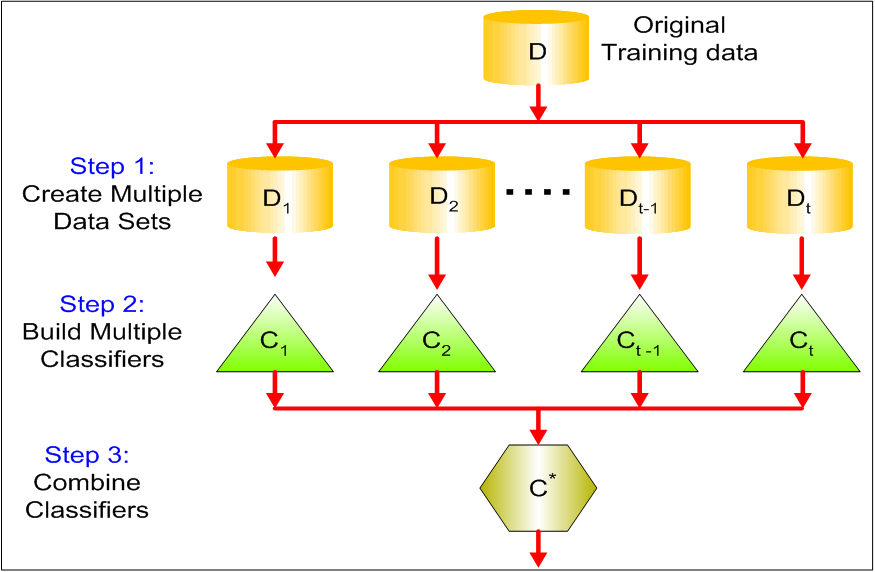
\includegraphics[width=0.6\linewidth,keepaspectratio]{ensmb}
\end{center}
\tiny{(Reference: Basics of Ensemble Learning Explained in Simple English - Tavish Shrivastava)}
\end{frame}

%%%%%%%%%%%%%%%%%%%%%%%%%%%%%%%%%%%%%%%%%%%%%%%%%%%%%%%%%%%%%%%%%%%%%%%%%%%%%%%%%%
\begin{frame}[fragile]\frametitle{}
\begin{center}
{\Large Ensemble Approaches}
\end{center}
\end{frame}

%%%%%%%%%%%%%%%%%%%%%%%%%%%%%%%%%%%%%%%%%%%%%%%%%%%%%%%%%%
\begin{frame}[fragile]\frametitle{Decision Tree Model Ensembles}
\begin{itemize}
\item Bagging
\item Boosting
\item Random Forests
\end{itemize}
\end{frame}

%%%%%%%%%%%%%%%%%%%%%%%%%%%%%%%%%%%%%%%%%%%%%%%%%%%%%%%%%%
\begin{frame}[fragile]\frametitle{Bagging (Bootstrapping)}
\begin{itemize}
\item Stands for {\bf B}ootstrap {\bf Agg}regat{\bf ing}
\item It was proposed by Leo Breiman in 1994.
\item A way to decrease the variance of your prediction
\item By generating additional data for training from your original data-set 
\item Using combinations with repetitions to produce multi-sets of the same cardinality/size as your original data.
\end{itemize}
\end{frame}

%%%%%%%%%%%%%%%%%%%%%%%%%%%%%%%%%%%%%%%%%%%%%%%%%%%%%%%%%%
\begin{frame}[fragile]\frametitle{Statistical Idea of Bootstrapping}
\begin{itemize}
\item Say, you have a complex distribution and you are asked to find its median.
\item If it was some standard distribution like Normal, then formulae are available
\item Here the trick is to sample, say randomly pick 10 points, and then find median of them.
\item Do this multiple times, say , 1000. You will have an array of medians. Find its median as answer.
\end{itemize}

\begin{center}
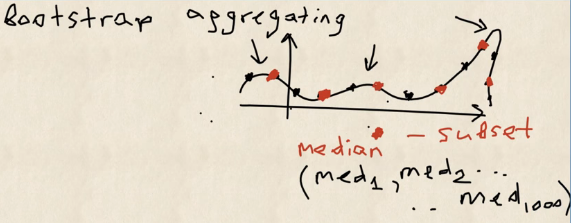
\includegraphics[width=0.5\linewidth,keepaspectratio]{ens11}
\end{center}
Bootstrap is used for Bagging.
\end{frame}


%%%%%%%%%%%%%%%%%%%%%%%%%%%%%%%%%%%%%%%%%%%%%%%%%%%%%%%%%%
\begin{frame}[fragile]\frametitle{Idea of Bagging}
\begin{itemize}
\item Let there be a sample $X$ of size $N$. 
\item We can make a new sample from the original sample by drawing N elements from the latter randomly and uniformly, with replacement. 
\item In other words, we select a random element from the original sample of size $N$ and do this $N$ times. 
\item All elements are equally likely to be selected, thus each element is drawn with the equal probability $\frac{1}{N}$.
\item Due to `With replacement' mode, in all cases total is always $N$.
\item Note that, because we put the balls back, there may be duplicates in the new sample. Let's call this new sample $X_1$
\end{itemize}
\end{frame}

%%%%%%%%%%%%%%%%%%%%%%%%%%%%%%%%%%%%%%%%%%%%%%%%%%%%%%%%%%
\begin{frame}[fragile]\frametitle{Bagging}
By repeating this procedure $M$ times, we create $M$ bootstrap samples $X_1, \dots, X_M$. 
In the end, we have a sufficient number of samples and can compute various statistics of the original distribution.

\begin{center}
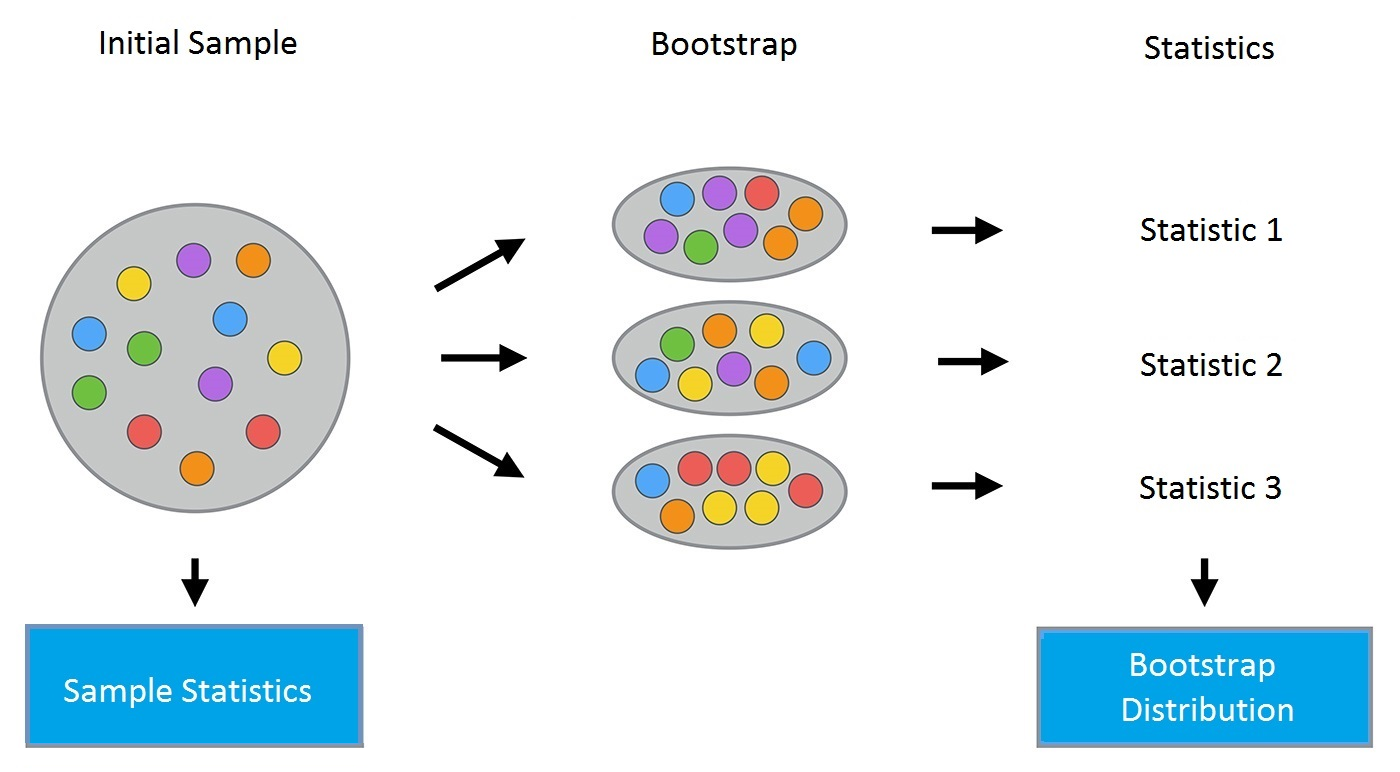
\includegraphics[width=0.6\linewidth,keepaspectratio]{ens8}
\end{center}

Distribution of the statistics (say, median) from each sample creates the Bootstrap distribution.

Condition for Bagging: Samples/rows must be idd (independently identically distributed)
\end{frame}


%%%%%%%%%%%%%%%%%%%%%%%%%%%%%%%%%%%%%%%%%%%%%%%%%%%%%%%%%%
\begin{frame}[fragile]\frametitle{Bagging}
\begin{center}
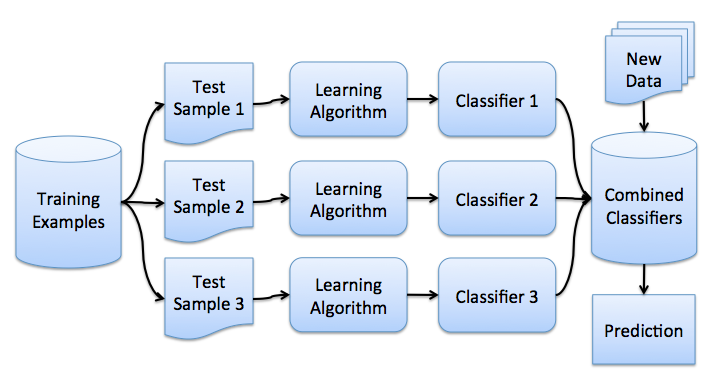
\includegraphics[width=\linewidth,keepaspectratio]{ens9}
\end{center}
\end{frame}






%%%%%%%%%%%%%%%%%%%%%%%%%%%%%%%%%%%%%%%%%%%%%%%%%%%%%%%%%%
\begin{frame}[fragile]\frametitle{Bagging}
\begin{itemize}
\item We train a number (ensemble) of decision trees from bootstrap samples of our training set. 
\item Bootstrap sampling means drawing random samples from our training set with replacement. 
\item E.g., if our training set consists of 7 training samples, our bootstrap samples
\end{itemize}
\begin{center}
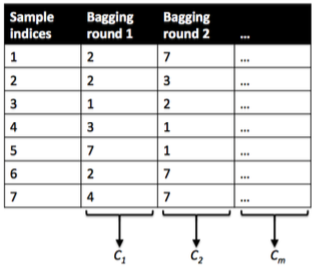
\includegraphics[width=0.4\linewidth,keepaspectratio]{ens1}
\end{center}
\end{frame}

%%%%%%%%%%%%%%%%%%%%%%%%%%%%%%%%%%%%%%%%%%%%%%%%%%%%%%%%%%
\begin{frame}[fragile]\frametitle{Bagging}
\begin{itemize}
\item After we trained our (m) decision trees, we can use them to classify new data via majority rule. 
\item For instance, we'd let each decision tree make a decision and predict the class label that received more votes. 
\item  Typically, this would result in a less complex decision boundary, and the bagging classifier would have a lower variance (less overfitting) than an individual decision tree. 
\end{itemize}

\end{frame}

%%%%%%%%%%%%%%%%%%%%%%%%%%%%%%%%%%%%%%%%%%%%%%%%%%%%%%%%%%
\begin{frame}[fragile]\frametitle{Bagging}
\begin{itemize}
\item Below is a plot comparing a single decision tree (left) to a bagging classifier (right) 
\end{itemize}
\begin{center}
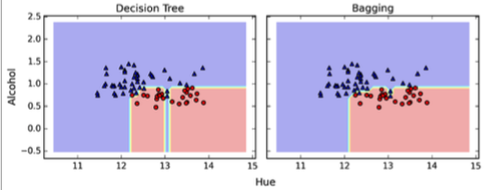
\includegraphics[width=0.7\linewidth,keepaspectratio]{ens2}
\end{center}
\tiny{(Reference: https://sebastianraschka.com/faq/docs/bagging-boosting-rf.html)}
\end{frame}


%
%%%%%%%%%%%%%%%%%%%%%%%%%%%%%%%%%%%%%%%%%%%%%%%%%%%%%%%%%%%
%\begin{frame}[fragile]\frametitle{Bagging}
%\begin{itemize}
%\item Ensemble method that ``manipulates the training set''
%\item Action: repeatedly sample with replacement according to uniform probability distribution
%\item Every instance has equal chance of being picked
%\item Some instances may be picked multiple times; others may not be chosen
%\item Sample Size: same as training set
%\end{itemize}
%\end{frame}
%
%%%%%%%%%%%%%%%%%%%%%%%%%%%%%%%%%%%%%%%%%%%%%%%%%%%%%%%%%%%
%\begin{frame}[fragile]\frametitle{Bagging Algorithm}
%\begin{itemize}
%\item Di: each bootstrap sample
%\item Footnote: also called bootstrap aggregating
%\item On average, each Di will contain 63\% of original training data.;
%Probability of sample being selected for Di: 1 - (1 - (1/N)N;
%Converges to: 1 - 1/e = 0.632 ;
%\item Consequently, every bootstrap sample will be missing some of the instances from the dataset so each bootstrap sample will be different and this means that models trained on different bootstrap samples will also be different 
%
%\end{itemize}
%%\begin{center}
%%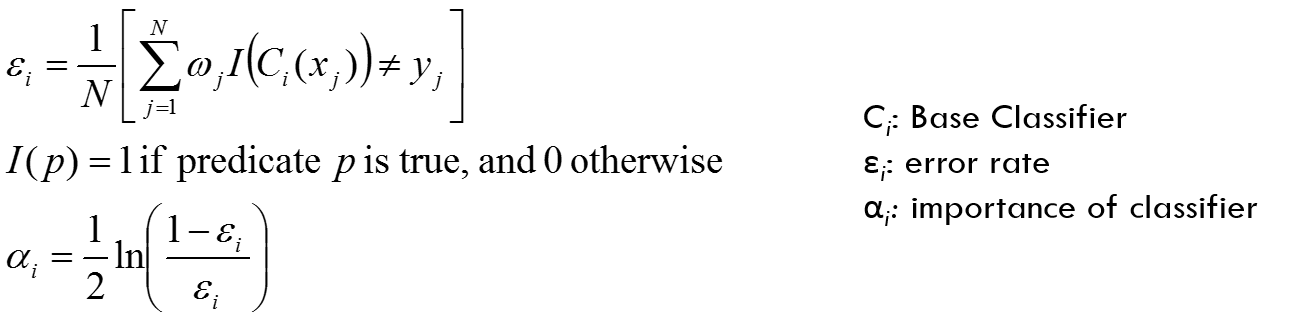
\includegraphics[width=\linewidth,keepaspectratio]{adaboost}
%%\end{center}
%
%\end{frame}

%%%%%%%%%%%%%%%%%%%%%%%%%%%%%%%%%%%%%%%%%%%%%%%%%%%%%%%%%%
\begin{frame}[fragile]\frametitle{Boosting}
\begin{itemize}
\item Takes a random sample from training set
\item Trains a model
\item Uses original data from Training to test how good this new model is.
\item For the next model, when we chose sample from the training set, the points which got mis-classified previously are weighted more to be picked up now.
\item Train the next model.
\item We test both models together by assembling their individual output.
\end{itemize}
\end{frame}


%%%%%%%%%%%%%%%%%%%%%%%%%%%%%%%%%%%%%%%%%%%%%%%%%%%%%%%%%%
\begin{frame}[fragile]\frametitle{Boosting}
\begin{itemize}
\item In contrast to bagging, we use very simple classifiers as base classifiers, so-called ''weak learners.'' 
\item Picture these weak learners as ''decision tree stumps'' -- decision trees with only 1 splitting rule. 
\end{itemize}
\end{frame}

%%%%%%%%%%%%%%%%%%%%%%%%%%%%%%%%%%%%%%%%%%%%%%%%%%%%%%%%%%
\begin{frame}[fragile]\frametitle{Boosting}
\begin{itemize}
\item We start with one decision tree stump (1) and "focus" on the samples it got wrong. 
\item In the next round, we train another decision tree stump that attempts to get these samples right (2);
\item Again, this 2nd classifier will likely get some other samples wrong, so do it one more time
\end{itemize}
\begin{center}
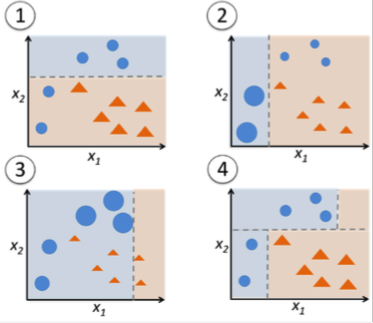
\includegraphics[width=0.4\linewidth,keepaspectratio]{ens3}
\end{center}
\end{frame}



%%%%%%%%%%%%%%%%%%%%%%%%%%%%%%%%%%%%%%%%%%%%%%%%%%%%%%%%%%%
%\begin{frame}[fragile]\frametitle{Boosting}
%\begin{itemize}
%\item A two-step approach
%\item First uses subsets of the original data to produce a series of averagely performing models
%\item Then ''boosts'' their performance by combining them together using a particular cost function (=majority vote).
%\end{itemize}
%\end{frame}


%%%%%%%%%%%%%%%%%%%%%%%%%%%%%%%%%%%%%%%%%%%%%%%%%%%%%%%%%%
\begin{frame}[fragile]\frametitle{Boosting}
\begin{itemize}
\item Unlike bagging, in the classical boosting the subset creation is not random and depends upon the performance of the previous models
\item Every new subsets contains the elements that were (likely to be) misclassified by previous models.
\end{itemize}
\end{frame}


%%%%%%%%%%%%%%%%%%%%%%%%%%%%%%%%%%%%%%%%%%%%%%%%%%%%%%%%%%
\begin{frame}[fragile]\frametitle{Boosting}
\begin{itemize}
\item Boosting works by iteratively creating models and adding them to the ensemble
\item Iteration stops when a predefined number of models have been added
\item Each new model added to the ensemble is biased to pay more attention to instances that previous models mis-classified (weighted dataset). 
\end{itemize}
\end{frame}
%
%%%%%%%%%%%%%%%%%%%%%%%%%%%%%%%%%%%%%%%%%%%%%%%%%%%%%%%%%%%
%\begin{frame}[fragile]\frametitle{Boosting}
%\begin{itemize}
%\item Initially instances are assigned weights of 1/N
%\item Each is equally likely to be chosen for sample
%\item Sample drawn with replacement: Di
%\item Classifier induced on Di
%\item Weights of training examples are updated:
%\item Instances classified incorrectly have weights increased
%\item Instances classified correctly have weights decreased
%\end{itemize}
%\end{frame}

%%%%%%%%%%%%%%%%%%%%%%%%%%%%%%%%%%%%%%%%%%%%%%%%%%%%%%%%%%%
%\begin{frame}[fragile]\frametitle{Boosting}
%During each iteration the algorithm: 
%
%\begin{itemize}
%\item Induces a model and calculates the total error, $\epsilon$, by summing the weights of the training instances for which the predictions made by the model are incorrect. 
%\item Increases the weights for the instances misclassified 
%\item Decreases the weights for the instances correctly classified
%\item Calculate a confidence factor $\alpha$, for the model such that $\alpha$ increases as $\epsilon$ decreases
%
%\end{itemize}
%\end{frame}

%%%%%%%%%%%%%%%%%%%%%%%%%%%%%%%%%%%%%%%%%%%%%%%%%%%%%%%%%%
\begin{frame}[fragile]\frametitle{Boosting Example}
\begin{center}
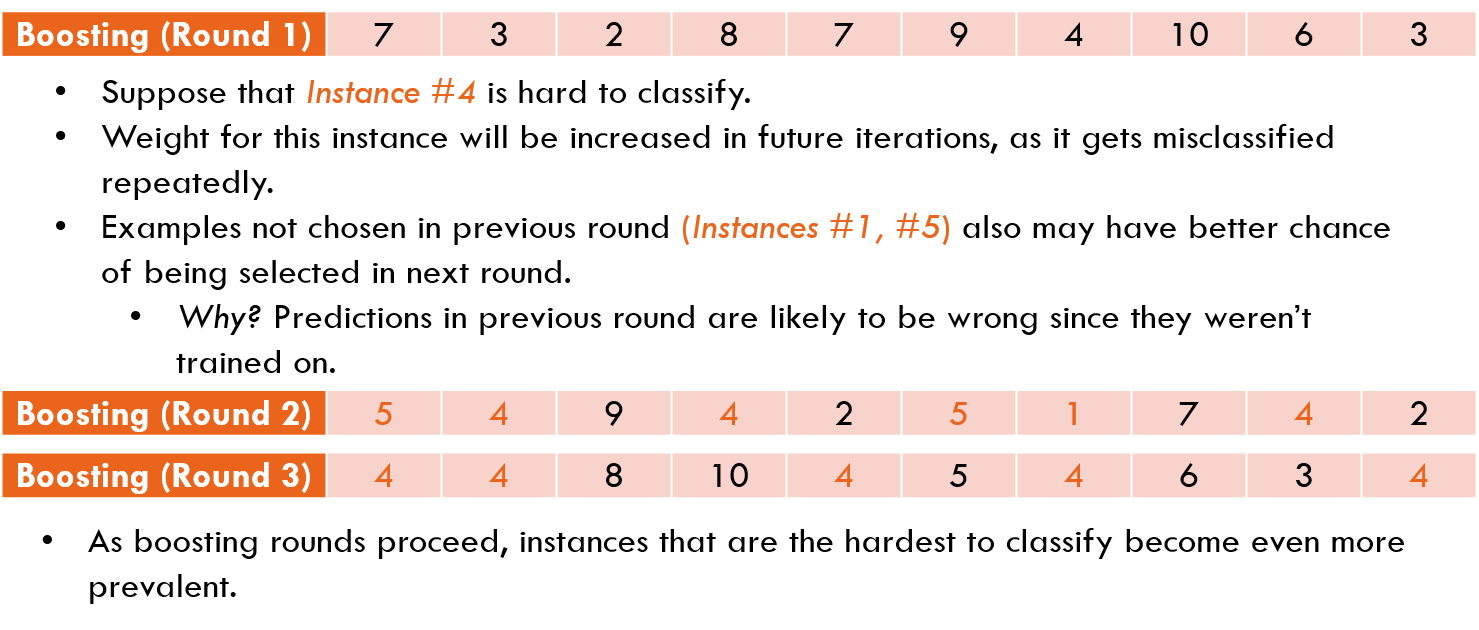
\includegraphics[width=\linewidth,keepaspectratio]{boost}
\end{center}

\end{frame}

%%%%%%%%%%%%%%%%%%%%%%%%%%%%%%%%%%%%%%%%%%%%%%%%%%%%%%%%%%
\begin{frame}[fragile]\frametitle{Prediction}
\begin{itemize}
\item Once the set of models have been created the ensemble makes predictions using a weighted aggregate of the predictions made by the individual models. 
\item The weights used in this aggregation are simply the confidence factors associated with each model. 
\item Several different boosting algorithms exist
\item Different by:
\begin{itemize}
\item How weights of training instances are updated after each boosting round
\item How predictions made by each classifier are combined. Each boosting round produces one base classifier
\end{itemize}
\end{itemize}
\end{frame}

%%%%%%%%%%%%%%%%%%%%%%%%%%%%%%%%%%%%%%%%%%%%%%%%%%%%%%%%%%
\begin{frame}[fragile]\frametitle{AdaBoost}
\begin{itemize}
\item AdaBoost is a popular boosting algorithm
\item "Adaptive" or "incremental" learning from mistakes.
\item Eventually, we will come up with a model that has a lower bias than an individual decision tree (thus, it is less likely to underfit the training data)
\end{itemize}
\begin{center}
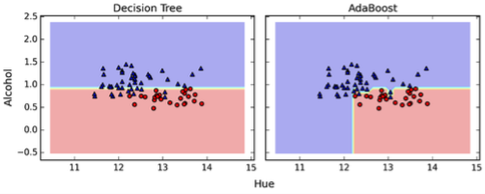
\includegraphics[width=0.8\linewidth,keepaspectratio]{ens4}
\end{center}

\end{frame}



%%%%%%%%%%%%%%%%%%%%%%%%%%%%%%%%%%%%%%%%%%%%%%%%%%%%%%%%%%
\begin{frame}[fragile]\frametitle{Bagging vs. Boosting}
\begin{itemize}
\item Boosting: Sample with nonuniform distribution
\item Unlike bagging where each instance had equal chance of being selected
\item Boosting Motivation: focus on instances that are harder to classify
\item How: give harder instances more weight in future rounds
\end{itemize}
\end{frame}

%%%%%%%%%%%%%%%%%%%%%%%%%%%%%%%%%%%%%%%%%%%%%%%%%%%%%%%%%%
\begin{frame}[fragile]\frametitle{Bagging (recap)}
\begin{itemize}
\item Parallel ensemble: each model is built independently
\item Aim to decrease variance, not bias
\item Suitable for high variance low bias models (complex models)
\item An example of a tree based method is random forest, which develop fully grown trees (note that RF modifies the grown procedure to reduce the correlation between trees)
\end{itemize}

\end{frame}

%%%%%%%%%%%%%%%%%%%%%%%%%%%%%%%%%%%%%%%%%%%%%%%%%%%%%%%%%%
\begin{frame}[fragile]\frametitle{Bagging (recap)}

\begin{center}
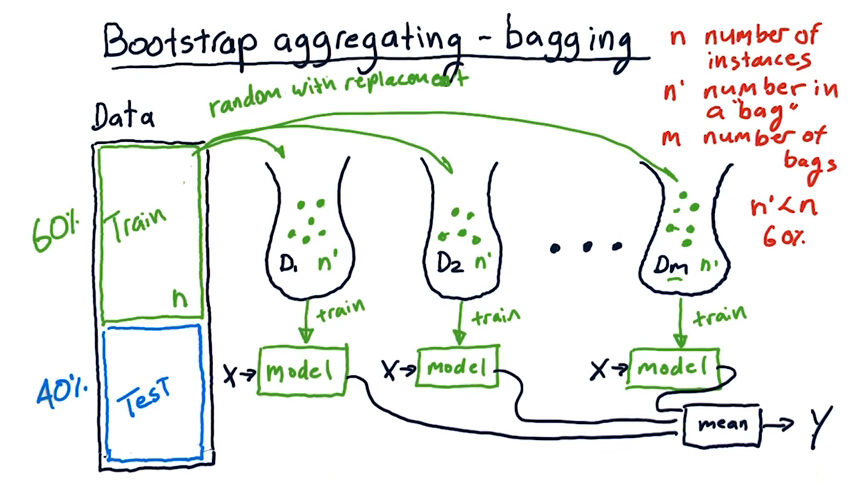
\includegraphics[width=0.8\linewidth,keepaspectratio]{ens5}
\end{center}
\tiny{(Reference: Bootstrap aggregating bagging - Udacity)}
\end{frame}

%%%%%%%%%%%%%%%%%%%%%%%%%%%%%%%%%%%%%%%%%%%%%%%%%%%%%%%%%%
\begin{frame}[fragile]\frametitle{Boosting (recap)}
\begin{itemize}
\item Sequential ensemble: try to add new models that do well where previous models lack
\item Aim to decrease bias, not variance
\item Suitable for low variance high bias models
\item An example of a tree based method is gradient boosting
\end{itemize}

\end{frame}

%%%%%%%%%%%%%%%%%%%%%%%%%%%%%%%%%%%%%%%%%%%%%%%%%%%%%%%%%%
\begin{frame}[fragile]\frametitle{Boosting (recap)}

\begin{center}
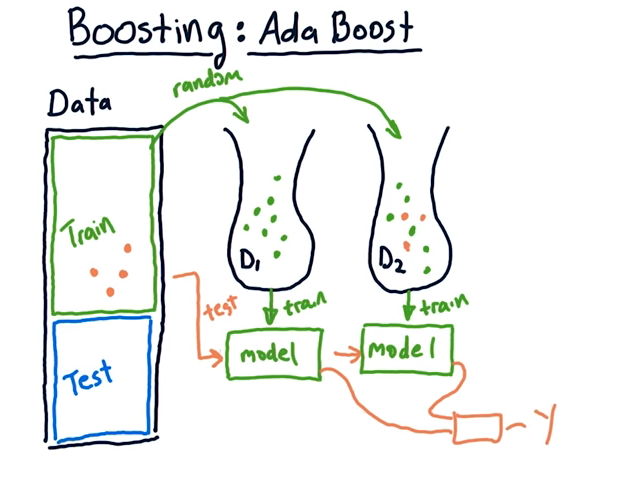
\includegraphics[width=0.8\linewidth,keepaspectratio]{ens6}
\end{center}
\tiny{(Reference: Bootstrap aggregating bagging - Udacity)}
\end{frame}


%
%%%%%%%%%%%%%%%%%%%%%%%%%%%%%%%%%%%%%%%%%%%%%%%%%%%%%%%%%%%
%\begin{frame}[fragile]\frametitle{Ensemble Method Performance on Classic Data Sets}
%\begin{center}
%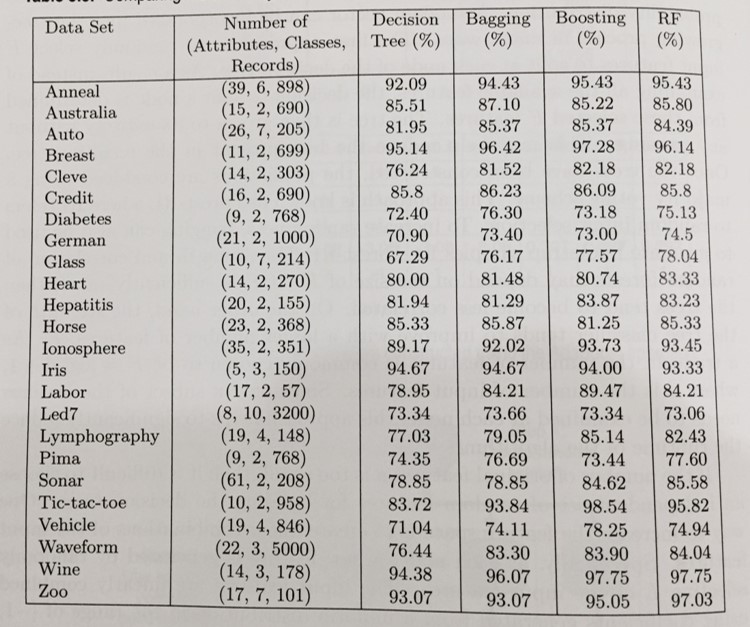
\includegraphics[width=0.8\linewidth,keepaspectratio]{ensclass}
%\end{center}
%\end{frame}



%%%%%%%%%%%%%%%%%%%%%%%%%%%%%%%%%%%%%%%%%%%%%%%%%%%%%%%%%%
\begin{frame}[fragile]\frametitle{Ensemble Choices}
\begin{itemize}
\item Which approach should we use? 
\item Bagging is simpler to implement and parallelize than boosting and, so, may be better with respect to ease of use and training time.
\end{itemize}
\end{frame}


%%%%%%%%%%%%%%%%%%%%%%%%%%%%%%%%%%%%%%%%%%%%%%%%%%%%%%%%%%
\begin{frame}[fragile]\frametitle{Ensemble Choices}
Empirical results indicate: 
\begin{itemize}
\item Boosted decision tree ensembles were the best performing model of those tested for datasets containing up to 4,000 descriptive features.
\item Random forest ensembles (based on bagging) performed better for datasets containing more that 4,000 features. 
\end{itemize}

\end{frame}



%%%%%%%%%%%%%%%%%%%%%%%%%%%%%%%%%%%%%%%%%%%%%%%%%%%%%%%%%%
\begin{frame}[fragile]\frametitle{Ensemble Methods (Recap)}

\begin{center}
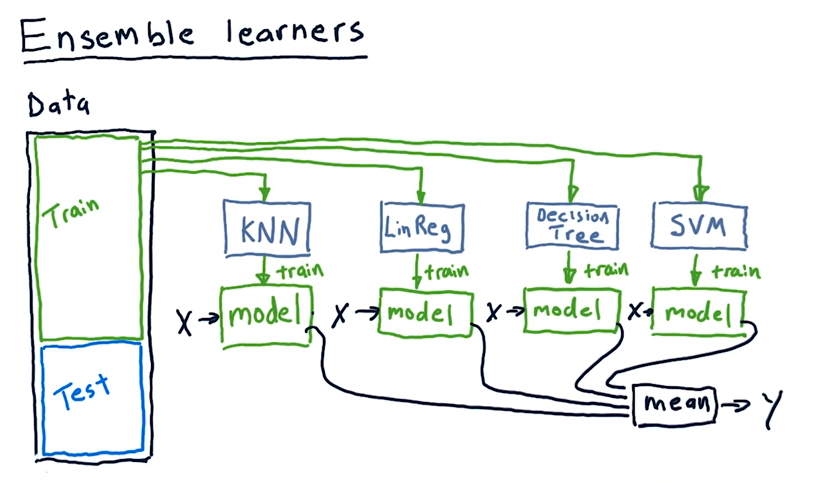
\includegraphics[width=0.8\linewidth,keepaspectratio]{ens7}
\end{center}
\tiny{(Reference: Bootstrap aggregating bagging - Udacity)}
\end{frame}


%%%%%%%%%%%%%%%%%%%%%%%%%%%%%%%%%%%%%%%%%%%%%%%%%%%%%%%%%%
\begin{frame}[fragile]\frametitle{Ensemble Methods (Recap)}
\begin{itemize}
\item Advantages:
\begin{itemize}
\item Astonishingly good performance
\item Modeling human behavior: making judgment based on many trusted advisors, each with their own specialty
\end{itemize}
\item Disadvantage:
\begin{itemize}
\item Combined models rather hard to analyze. Tens or hundreds of individual models
\item Current research: making models more comprehensible
\end{itemize}
\end{itemize}
\end{frame}
